\documentclass{beamer}

\mode<presentation>
{
  %\usetheme{AnnArbor}
  \usetheme{Montpellier}
  %\usetheme{Hannover}
  %\usetheme{Singapore}
  %\usetheme{Madrid}
}

\newcommand*\oldmacro{}
\let\oldmacro\insertshorttitle% ursprüngliche Definition sichern
\renewcommand*\insertshorttitle{%
  \oldmacro
  \hfill\insertframenumber\,/\,\inserttotalframenumber}

\setbeamertemplate{navigation symbols}{}

\usepackage[german]{babel}

%\usepackage[latin1]{inputenc}
\usepackage[utf8]{inputenc}

\usepackage{hyperref}

% WTF? times? serious?
%\usepackage{times}
\usepackage[T1]{fontenc}

\usepackage{listings}

\usepackage{tabularx}
\newcolumntype{L}[1]{>{\raggedright\arraybackslash}p{#1}}

\title[Project Proposal]{Advanced Rendering \\ Project Proposal}

%\subtitle {Untertitel} (optional)

\author[Brauer, Heppner, Koza]
{S. Brauer \and S. Heppner \and A. Koza}

\institute[University of Paderborn]{Institute for Computer Science}

\date{\today}


\subject{Computer Science}

\pgfdeclareimage[height=0.5cm]{university-logo}{figures/upb_logo.png}
\logo{\pgfuseimage{university-logo}}



% Folgendes sollte gelöscht werden, wenn man nicht am Anfang jedes
% Unterabschnitts die Gliederung nochmal sehen möchte.
%\AtBeginSubsection[]
%{
%  \begin{frame}<beamer>{Gliederung}
%    \tableofcontents[currentsection,currentsubsection]
%  \end{frame}
%}



\begin{document}

\begin{frame}
  \titlepage
\end{frame}

\begin{frame}{Idea}
	\begin{itemize}
		\item Model inner courtyard of university in detail
		\begin{itemize}
			\item Fountain
			\item Clock
			\item Vegetation
		\end{itemize}
	\end{itemize}	
\end{frame}

\begin{frame}{Texturing and Illumination Effects}
	\begin{itemize}
		\item Normal Mapping
		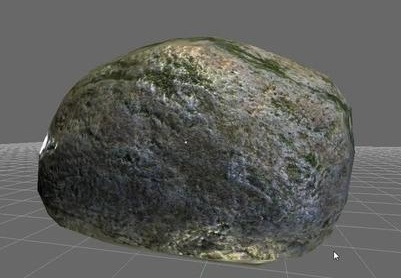
\includegraphics[height=2cm]{figures/normal_map_stone.jpg}
		\item Ambient Occlusion
	\end{itemize}
\end{frame}

\begin{frame}{Image-Based Effects}
	\begin{itemize}
		\item Skyboxes
		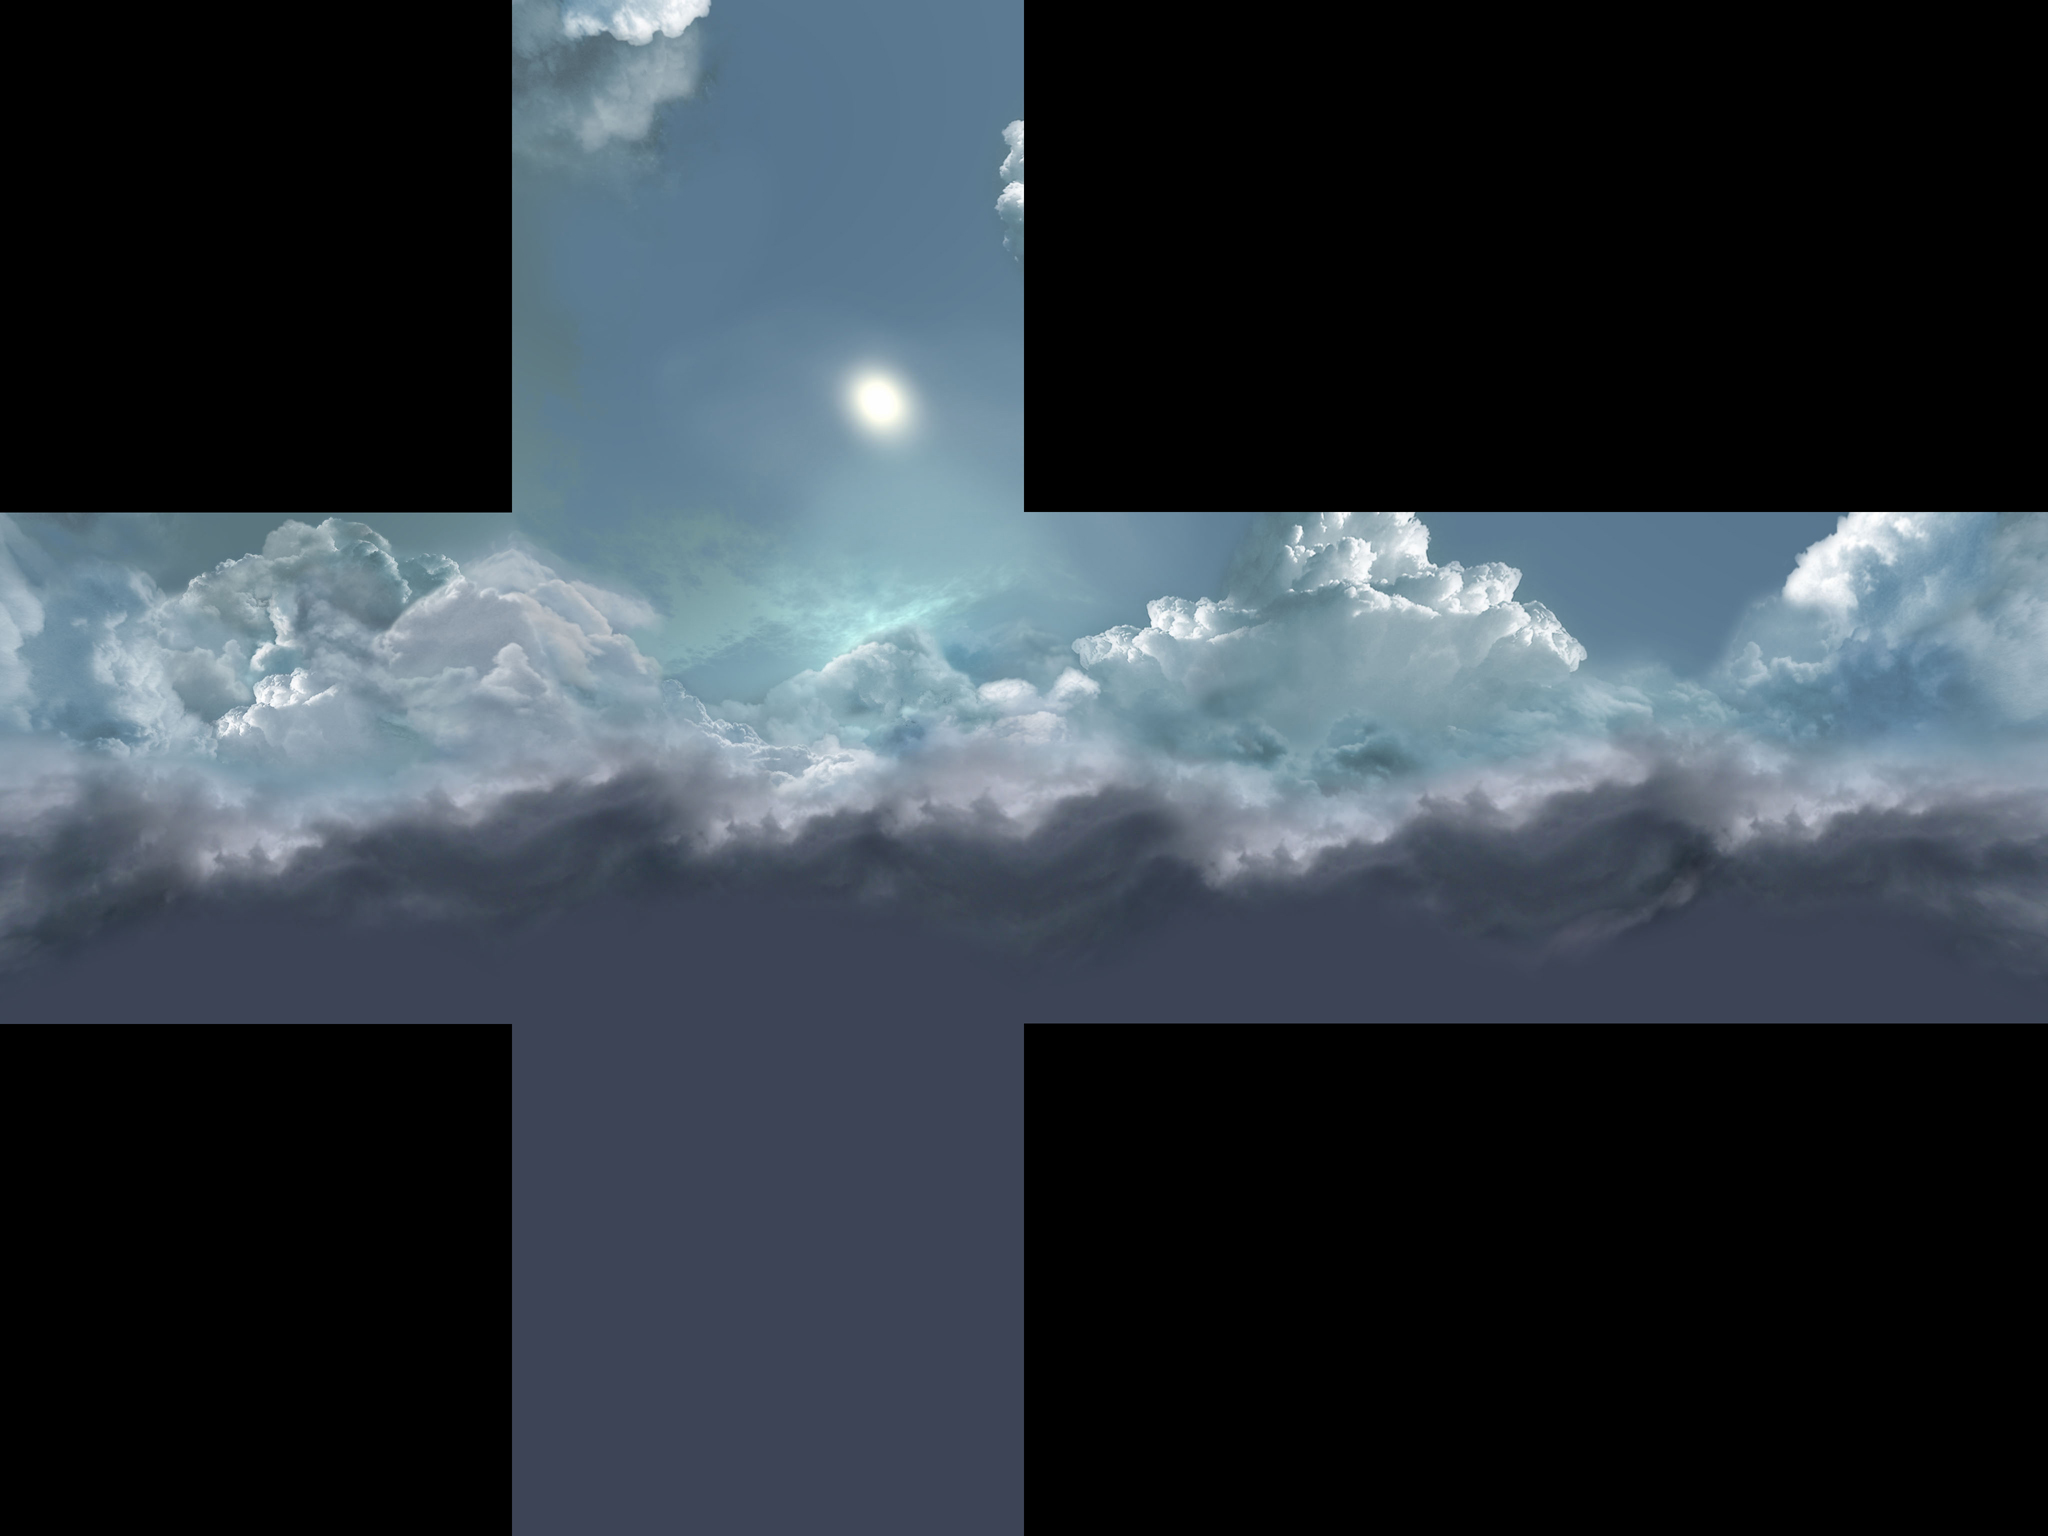
\includegraphics[height=2cm]{figures/skybox.jpg}
		\item Lens Flare
		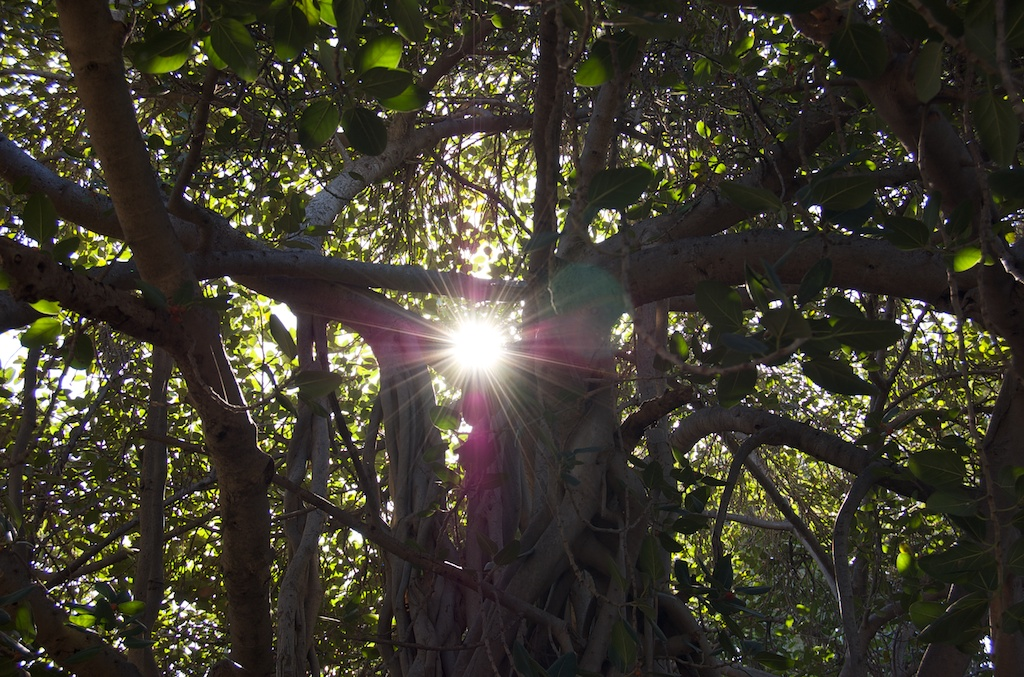
\includegraphics[height=2cm]{figures/lens_flare_tree.jpg}
		\item Bloom
		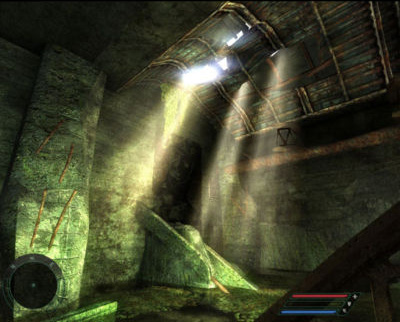
\includegraphics[height=2cm]{figures/bloom.jpg}
	\end{itemize}
\end{frame}

\begin{frame}{Non-Photorealistic Rendering}
	\begin{itemize}
		\item Toon-Shader gets activated at some point in time and
		\item Every object is smoothly converted and looks like in a carton
	\end{itemize}
	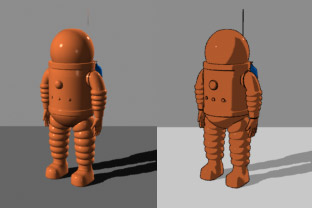
\includegraphics[height=2cm]{figures/toon_shader.jpg}
\end{frame}


\end{document}
